\subsection{Motion Node}\label{sec:motionnode}

\subsubsection{Event-Driven Data Flow}

Motion data propagation across the graph is coordinated through a publisher-subscriber model, in which nodes assume complementary roles as Motion Senders and Motion Receivers.
When a Motion Sender (an upstream node) completes its update, it triggers an \texttt{OnUpdate} event that downstream nodes subscribe to.
Motion Receivers subscribe to that event, read views from the shared buffer in a zero-copy manner, invoke their internal logic, write their transformations back into their own buffer, and then publish their \texttt{OnUpdate} as a Motion Sender (see Figure~\ref{fig:systemdesign} (b)).
This event-driven architecture provides several key advantages: loose coupling between nodes enhances reusability and isolation; encapsulation ensures that each node remains functionally coherent; compositional flexibility allows runtime pipelines to be dynamically assembled from interchangeable parts. 
This also guarantees extensibility where new nodes can be added without modifying existing ones.

\subsubsection{Data Access via Kinematic Buffer}
Next, we specify how nodes read and write motion data.
Each Motion Node writes joint data as whole or partial body pose samples into a generic \texttt{Kinematic Buffer}.
The buffer uses contiguous storage of translations, rotations, and optional joint attributes in a fixed human-body layout to keep data coherent across the DAG.
Zero-copy sharing across different body representations is achieved via lightweight Views and precomputed Slices over the same storage. 
A View exposes semantic joint layouts and contiguous index maps for body, hands, and fingers.
A Slice is a pre-resolved index set for joint subsets that gives O(1) access to. 
{\bf Figure~\ref{fig:kinematic-buffer}} shows nodes reading KinematicBufferView while maintaining a single contiguous storage.

\begin{figure}[t]
    \centering
    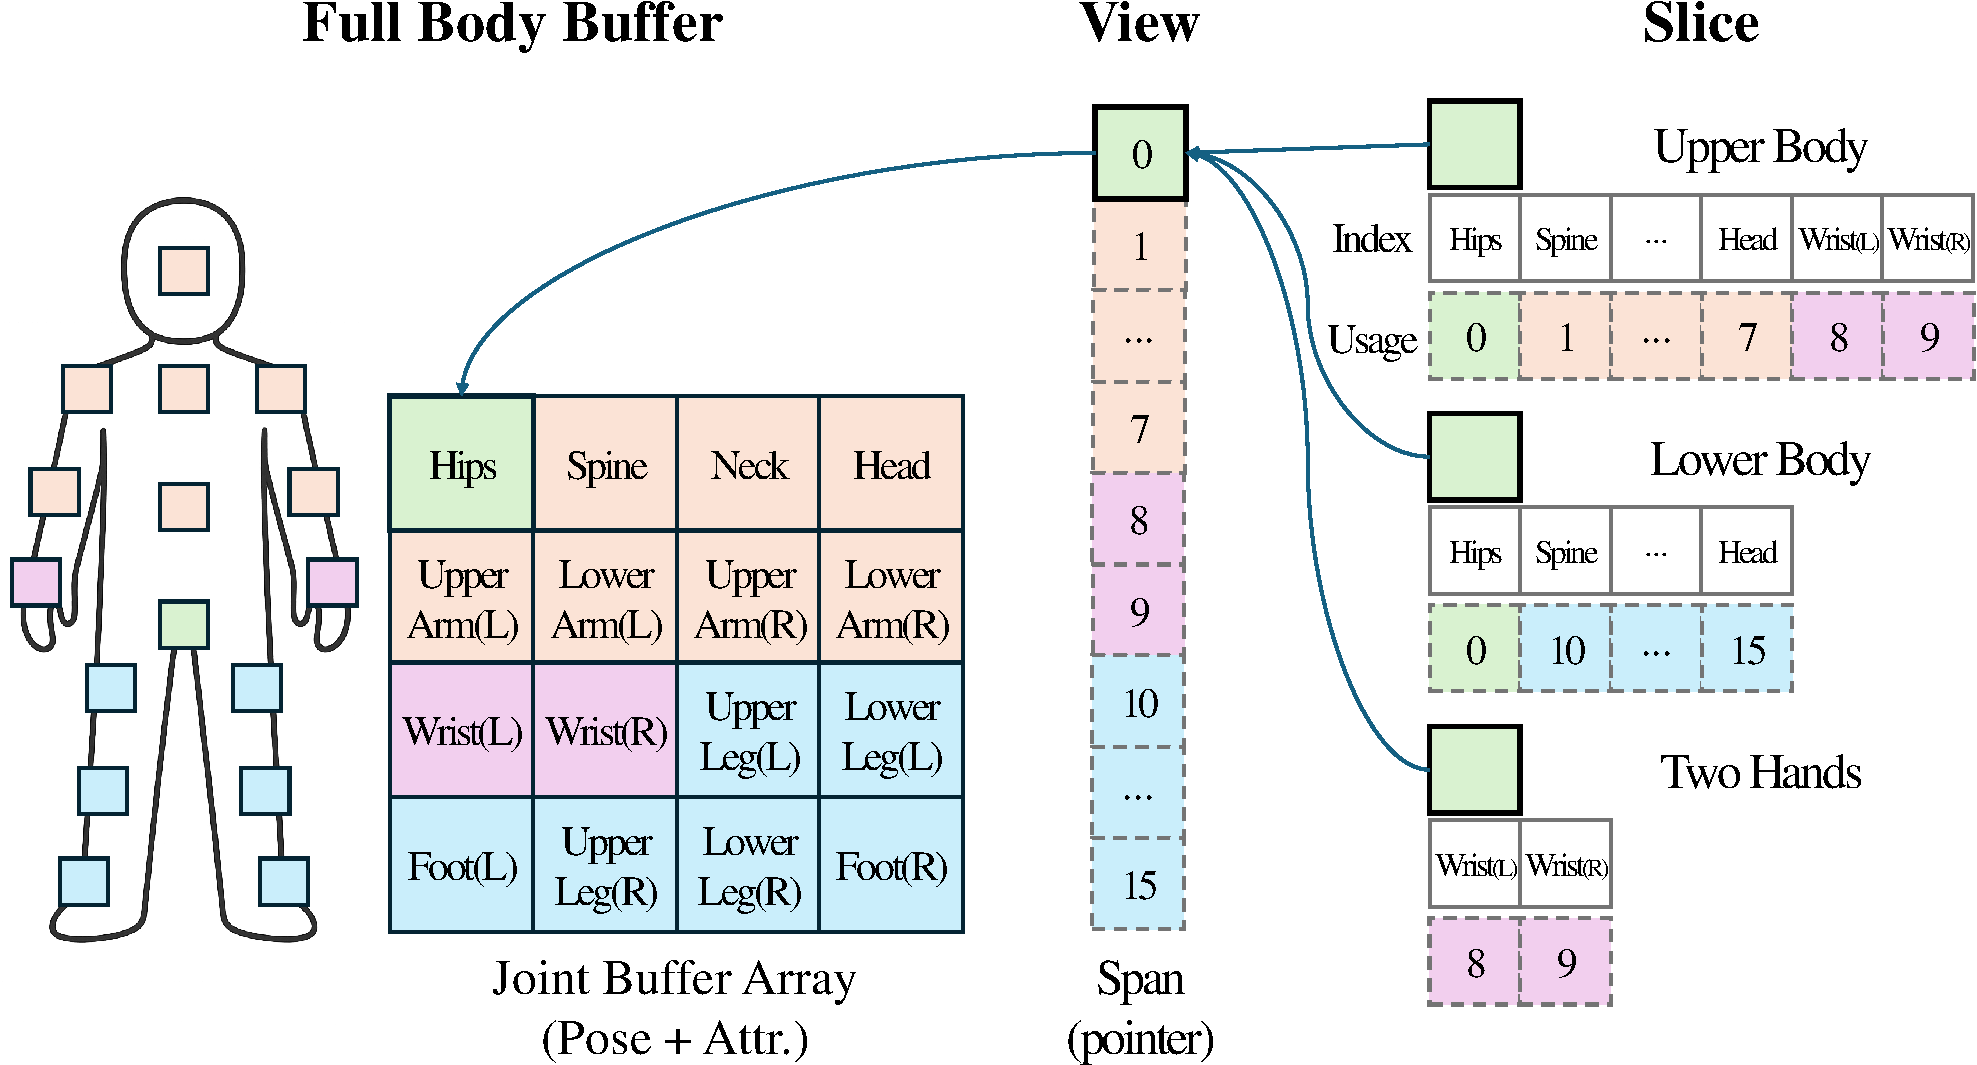
\includegraphics[width=0.95\columnwidth]{figures/fig2-kinematicbuffer.pdf}
    \caption{Kinematic Buffer memory layout with zero-copy views and slices for efficient joint data access across different body type representations.}
    \label{fig:kinematic-buffer}
\end{figure}

\subsubsection{Motion Trigger \& Retargeter}
The Motion Trigger and Retargeter define the entry and exit of the end-to-end pipeline, bridging tracking devices to the final avatar rig.
The Motion Trigger is a specialized Motion Sender that emits the initial pose sample and starts propagation through the pipeline. 
By implementing the Motion Sender interface, Motion Triggers bootstrap the event-driven flow and establish the first \texttt{OnUpdate} events.
Any component implementing the Motion Trigger interface therefore acts as an entry point that injects motion data into the pipeline.
In practice the system ships two primary triggers: the tracking manager and waypoint manager, which gather pose input from XR hardware and user-authored keyframes, respectively, before pushing those samples downstream.

Conversely, the Retargeter is a specialized Motion Receiver that bridges motion nodes to the avatar rig.
Each Retargeter reads processed motion data from the Kinematic Buffer, remaps it into the avatar's coordinate frame, and writes rig-specific transforms.
This final stage adapts the motion representation to each avatar.